\documentclass[UTF8]{article}
\usepackage{graphicx}
\usepackage{subfigure}
\usepackage{amsmath}
\usepackage{makecell}
\usepackage[utf8]{inputenc}
\usepackage[space]{ctex} %中文包
\usepackage{listings} %放代码
\usepackage{xcolor} %代码着色宏包
\usepackage{CJK} %显示中文宏包
\usepackage{float}
\usepackage{diagbox}
\usepackage{bm}
\usepackage{ulem} 
\usepackage{amssymb}
\usepackage{soul}
\usepackage{color}
\usepackage{geometry}
\usepackage{fancybox} %花里胡哨的盒子
\usepackage{xhfill} %填充包, 可画分割线 https://www.latexstudio.net/archives/8245
\usepackage{multicol} %多栏包
\usepackage{enumerate} %可以方便地自定义枚举标题
\usepackage{multirow} %表格中多行单元格合并
\usepackage{wasysym} %可以使用wasysym里的一堆奇奇怪怪的符号
\usepackage{hyperref} % url
%%%%%%%%%%%%%%%伪代码%%%%%%%%%%%%%%%
\usepackage{amsmath}
\usepackage{algorithm}
\usepackage{algorithmicx}
\usepackage[noend]{algpseudocode}
%%%%%%%%%%%%%%%画图包%%%%%%%%%%%%%%%
\usepackage{tikz}
\usepackage{pgfplots} % http://pgfplots.sourceforge.net/gallery.html
\usetikzlibrary{pgfplots.patchplots} % 拟合支持
\usetikzlibrary{arrows,shapes,automata,petri,positioning,calc} % 状态图支持
\usetikzlibrary{arrows.meta} % 箭头
\usetikzlibrary{shadows} % 阴影支持
\usepackage{forest} % 画树

\geometry{left = 1.5cm, right = 1.5cm, top=1.5cm, bottom=2cm}

\definecolor{mygreen}{rgb}{0,0.6,0}
\definecolor{mygray}{rgb}{0.5,0.5,0.5}
\definecolor{mymauve}{rgb}{0.58,0,0.82}
\lstset{
	backgroundcolor=\color{white}, 
	%\tiny < \scriptsize < \footnotesize < \small < \normalsize < \large < \Large < \LARGE < \huge < \Huge
	basicstyle = \footnotesize,       
	breakatwhitespace = false,        
	breaklines = true,                 
	captionpos = b,                    
	commentstyle = \color{mygreen}\bfseries,
	extendedchars = false,
	frame = shadowbox, 
	framerule=0.5pt,
	keepspaces=true,
	keywordstyle=\color{blue}\bfseries, % keyword style
	language = C++,                     % the language of code
	otherkeywords={string}, 
	numbers=left, 
	numbersep=5pt,
	numberstyle=\tiny\color{mygray},
	rulecolor=\color{black},         
	showspaces=false,  
	showstringspaces=false, 
	showtabs=false,    
	stepnumber=1,         
	stringstyle=\color{mymauve},        % string literal style
	tabsize=4,          
	title=\lstname           
}

%\sum\nolimits_{j=1}^{M}   上下标位于求和符号的水平右端,
%\sum\limits_{j=1}^{M}   上下标位于求和符号的上下处,
%\sum_{j=1}^{M}  对上下标位置没有设定,会随公式所处环境自动调整。

%%%%%%%%%%%%%画图包%%%%%%%%%%%%%
\usepackage{tikz}
%%%%%%%%%%%%%好看的矩形%%%%%%%%%%%%%
\tikzset{
  rect1/.style = {
    shape = rectangle,% 指定样式
    minimum height=2cm,% 最小高度
    minimum width=4cm,% 最小宽度
    align = center,% 文字居中
    drop shadow,% 阴影
  }
}
%%%%%%%%%%%%%画图背景包%%%%%%%%%%%%%
\usetikzlibrary{backgrounds}

%%%%%%%%%%%%%在tikz中画一个顶点%%%%%%%%%%%%%
%%%%%%%%%%%%%#1:node名称%%%%%%%%%%%%%
%%%%%%%%%%%%%#2:位置%%%%%%%%%%%%%
%%%%%%%%%%%%%#3:标签%%%%%%%%%%%%%
\newcommand{\newVertex}[3]{\node[circle, draw=black, line width=1pt, scale=0.8] (#1) at #2{#3}}
%%%%%%%%%%%%%在tikz中画一条边%%%%%%%%%%%%%
\newcommand{\newEdge}[2]{\draw [black,very thick](#1)--(#2)}
%%%%%%%%%%%%%在tikz中放一个标签%%%%%%%%%%%%%
%%%%%%%%%%%%%#1:名称%%%%%%%%%%%%%
%%%%%%%%%%%%%#2:位置%%%%%%%%%%%%%
%%%%%%%%%%%%%#3:标签内容%%%%%%%%%%%%%
\newcommand{\newLabel}[3]{\node[line width=1pt] (#1) at #2{#3}}

%%%%%%%%%%%%%强制跳过一行%%%%%%%%%%%%%
\newcommand{\jumpLine} {\hspace*{\fill} \par}
%%%%%%%%%%%%%关键点指令,可用itemise替代%%%%%%%%%%%%%
\newcommand{\keypoint}[2]{$\bullet$\textbf{#1}\quad#2\par}
%%%%%%%%%%%%%<T>平均值表示%%%%%%%%%%%%%
\newcommand{\average}[1]{\left\langle #1\right\rangle }
%%%%%%%%%%%%%表格内嵌套表格%%%%%%%%%%%%%
\newcommand{\tabincell}[2]{\begin{tabular}{@{}#1@{}}#2\end{tabular}}
%%%%%%%%%%%%%大黑点item头%%%%%%%%%%%%%
\newcommand{\itemblt}{\item[$\bullet$]}
%%%%%%%%%%%%%大圈item头%%%%%%%%%%%%%
\newcommand{\itemc}{\item[$\circ$]}
%%%%%%%%%%%%%大星星item头%%%%%%%%%%%%%
\newcommand{\itembs}{\item[$\bigstar$]}
%%%%%%%%%%%%%右▷item头%%%%%%%%%%%%%
\newcommand{\itemrhd}{\item[$\rhd$]}
%%%%%%%%%%%%%定义为%%%%%%%%%%%%%
\newcommand{\defas}{=_{df}}
%%%%%%%%%%%%%偏导%%%%%%%%%%%%%
\newcommand{\partialx}[2]{\frac{\partial #1}{\partial #2}}
%%%%%%%%%%%%%蕴含%%%%%%%%%%%%%
\newcommand{\imp}{\rightarrow}
%%%%%%%%%%%%%上取整%%%%%%%%%%%%%
\newcommand{\ceil}[1]{\lceil#1\rceil}
%%%%%%%%%%%%%下取整%%%%%%%%%%%%%
\newcommand{\floor}[1]{\lfloor#1\rfloor}

%%%%%%%%%%%%%双线分割线%%%%%%%%%%%%%
\newcommand*{\doublerule}{\hrule width \hsize height 1pt \kern 0.5mm \hrule width \hsize height 2pt}
%%%%%%%%%%%%%双线中间可加东西的分割线%%%%%%%%%%%%%
\newcommand\doublerulefill{\leavevmode\leaders\vbox{\hrule width .1pt\kern1pt\hrule}\hfill\kern0pt }
%%%%%%%%%%%%%左大括号%%%%%%%%%%%%%
\newcommand{\leftbig}[1]{\left\{\begin{array}{l}#1\end{array}\right.}
%%%%%%%%%%%%%矩阵%%%%%%%%%%%%%
\newcommand{\mat}[2]{\left[\begin{array}{#1}#2\end{array}\right]}
%%%%%%%%%%%%%可换行圆角文本框%%%%%%%%%%%%%
\newcommand{\ovalboxn}[1]{\ovalbox{\tabincell{l}{#1}}}
%%%%%%%%%%%%%设置section的counter, 使从1开始%%%%%%%%%%%%%
\setcounter{section}{0}

%%%%%%%%%%%%%Colors%%%%%%%%%%%%%
\newcommand{\lightercolor}[3]{% Reference Color, Percentage, New Color Name
    \colorlet{#3}{#1!#2!white}
}
\newcommand{\darkercolor}[3]{% Reference Color, Percentage, New Color Name
    \colorlet{#3}{#1!#2!black}
}
\definecolor{aquamarine}{rgb}{0.5, 1.0, 0.83}
\definecolor{Seashell}{RGB}{255, 245, 238} %背景色浅一点的
\definecolor{Firebrick4}{RGB}{255, 0, 0}%文字颜色红一点的
\lightercolor{gray}{20}{lgray}
\newcommand{\hlg}[1]{
	\begingroup
		\sethlcolor{lgray}%背景色
		\textcolor{black}{\hl{\mbox{#1}}}%textcolor里面对应文字颜色
	\endgroup
}



\title{计算机网络 Lab1\\\Large DNS Relay}
\author{PB18111697 王章瀚}

\begin{document}
\maketitle
\tableofcontents
\newpage
\section{实验目标}
\subsection{任务描述}
\noindent 给定一个 config 文件, 其每行都是 一个 IP 地址和一个域名, 要求实现一个 DNS 服务器以满足下列要求:
\begin{itemize}
\item Intercept: 如果查询的域名在列表中, 且对应为 0.0.0.0, 那么回复时应当表明无此条目, 设置 rcode 为 3
\item Local Resolve: 如果查询的域名在列表中, 且对应有一个有意义的 IP 地址, 那么就正确地回复该 IP 地址
\item Relay: 如果域名不在列表中, 就传递该域名给真正的 DNS 服务器, 然后将其返回结果发回客户端
\end{itemize}
此外, 还要求
\begin{itemize}
\item 指出每个 query 中被查询的 name
\item query 处理的时长
\item 能够处理并发的请求
\end{itemize}

\subsection{测试方法}
\begin{itemize}
\item nslookup: for basic functionality
\item 浏览器: 过滤广告
\end{itemize}

\section{程序介绍}
\subsection{文件说明}
以下是代码文件结构:
\begin{figure}[H]
	\centering
	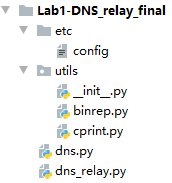
\includegraphics[width=\linewidth/5]{code_structure.png}
	\caption{代码文件结构}
\end{figure}\par
\begin{itemize}
\item utils.binrep: 用于 bytes, bin, binlist, int 等之间的相互转换, 主要是统一了一下函数名
\item utils.cprint: colorful printer, 用来方便地进行带颜色风格等的文字输出
\item dns: 用于解析 DNS 消息, 主要类包括 \hlg{DNSHeader}, \hlg{DNSQuestion}, \hlg{DNSAnswer}, 并提供了 \hlg{@property} 装饰器的参数访问方法, 提升了这些类的易用性.
\item dns\_relay: 主程序. 主要包括 \hlg{receiver}, \hlg{relay}, \hlg{forward}, \hlg{backsender} 这么几个函数. 通过 \hlg{multiprocessing} 的进程调度来协调他们.
\end{itemize}

\subsection{类与函数说明}
\subsubsection{dns.py}
\begin{itemize}
\item \hlg{DNSHeader}: 提供完整的 DNS header 访问与修改接口
\item \hlg{DNSQuestion}: 提供完整的 DNS question 访问与修改接口
\item \hlg{DNSAnswer}: 提供完整的 DNS answer 访问与修改接口
\end{itemize}
\subsubsection{dns\_relay.py}
\begin{itemize}
\item \hlg{receiver}: 带锁机制的接收器函数, 用以接收客户端的请求
\item \hlg{relay}: 进行请求解析, 根据其在 config 文件中的信息来决定如何返回
\item \hlg{forward}: 用以转发请求给真正的 DNS server, 从而获取真正的信息
\item \hlg{backsender}: 用以发回生成好的 answer
\end{itemize}
\section{程序设计特点}
\subsection{代码运行逻辑}
\begin{enumerate}[1. ]
\item 从\hlg{dns\_relay} 中的 \hlg{main} 函数开始运行程序
\item \hlg{main} 函数会创建一个共享队列和锁, 并作为参数传给新建的两个进程 \hlg{receiver} 和 \hlg{backsender}
\item \hlg{receiver} 负责接收请求, 并 start 一个新的进程以调用 \hlg{relay} 来处理该请求
\item 当一个请求被处理完后, 它的相关结果被放入共享队列中
\item \hlg{backsender} 不时检查队列内容, 如有内容则发送它们, 以将结果发回客户端
\end{enumerate}
\subsection{特殊功能设计}
\begin{itemize}
\item 彩色打印信息, 方便识别
\item 自动加载更新了的 config 文件, 避免重新启动程序
\item 相对完善的 except 处理
\item 信号量控制进程数, 防止管道使用占满
\end{itemize}

\section{程序运行过程与截图}
\subsection{环境配置}
\subsubsection{实验环境}
\begin{itemize}
\item Windows10
\item Python 3.7
\item Microsoft Edge 浏览器
\end{itemize}
\subsection{实验配置}
\subsubsection{设置 DNS 服务器}
\noindent 为了让 DNS 请求都经过我的 DNS 服务器, 需要做如下配置
\begin{figure}[H]
	\centering
	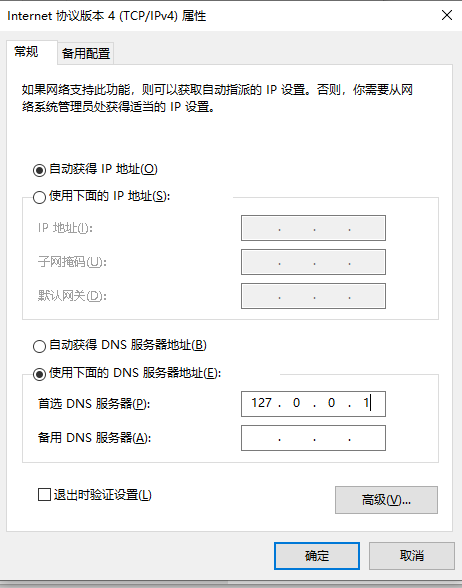
\includegraphics[width=\linewidth/2]{configdns.png}
	\caption{代码文件结构}
\end{figure}\par
\subsubsection{清空 DNS 缓存}
\noindent 只需要在命令行中运行 "\hlg{ipconfig /flushdns}" 即可
\subsubsection{清空浏览器缓存}
\noindent 就一些平时常做的操作, 这里就不截图了.
\subsection{nslookup}
\noindent 根据要求, 考虑以下配置:
\begin{figure}[H]
	\centering
	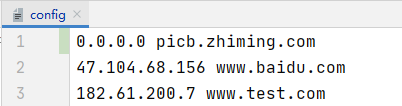
\includegraphics[width=\linewidth/2]{nslookup_config.png}
	\caption{nslookup 测试的 config 文件}
\end{figure}\par
\begin{itemize}
\item 查询 \hlg{www.test.com} 的结果: 可以从下图看出, 当发现 www.test.com 是 config 文件中配置了的, 并且请求类型为 A 类时, 就能够正确地返回指定的 182.61.200.7. 但当请求为 AAAA 类时, 则进行转发(relay).
\begin{figure}[H]
	\centering
	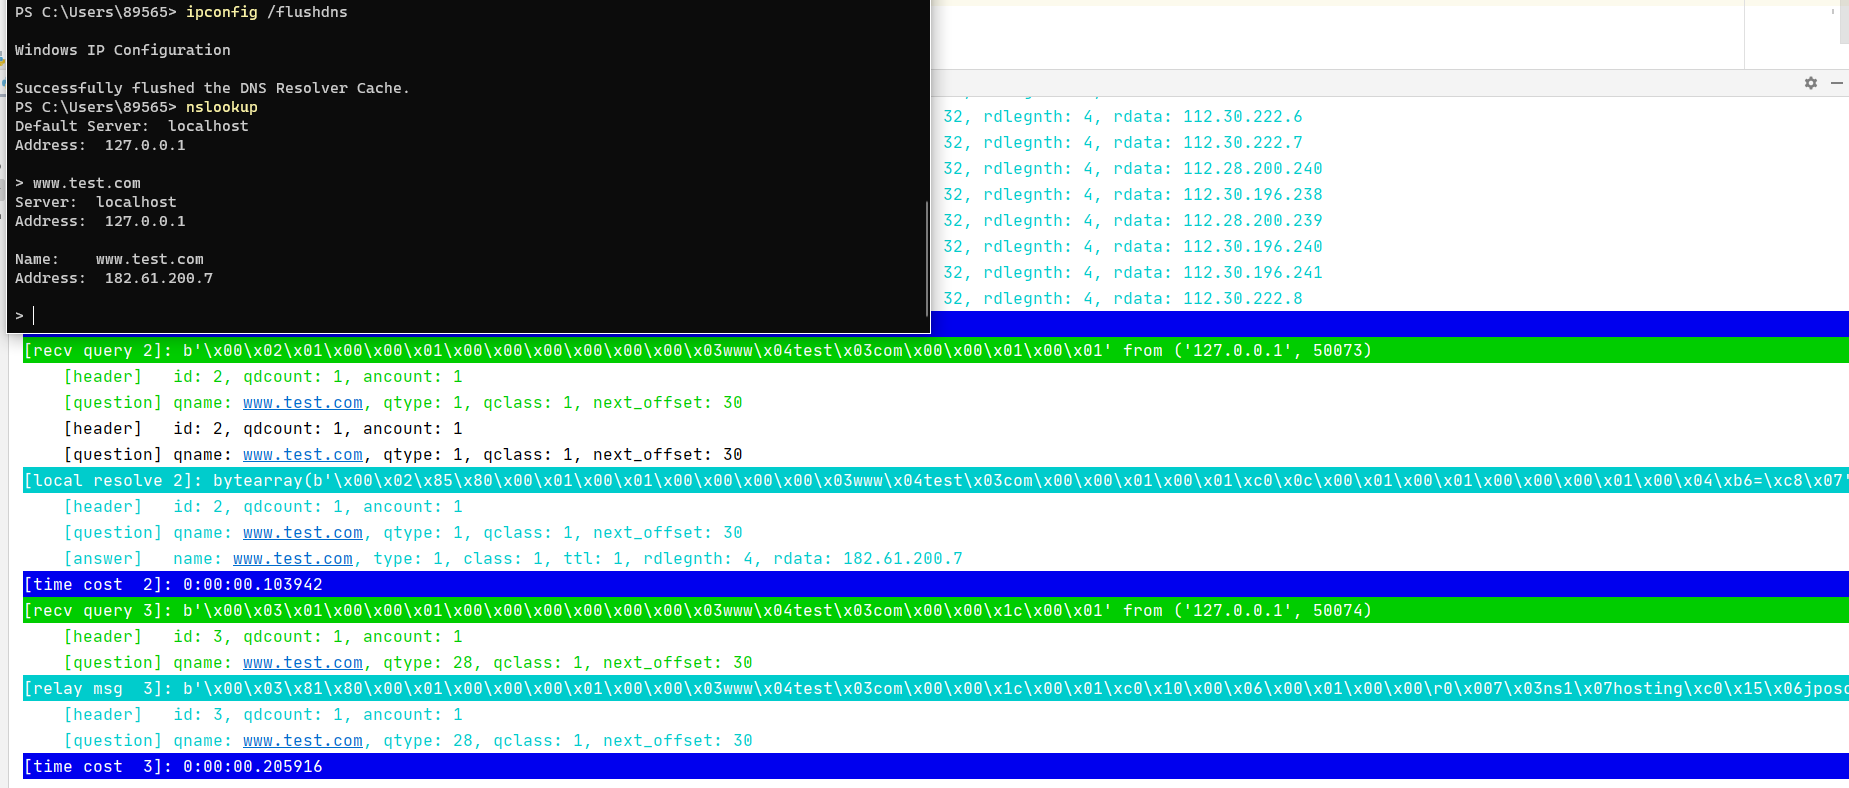
\includegraphics[width=\linewidth/9*8]{nsl_test.png}
	\caption{nslookup 查询 www.test.com 的结果}
\end{figure}\par
\item 查询 \hlg{www.baidu.com} 的结果: 类似上一个.
\begin{figure}[H]
	\centering
	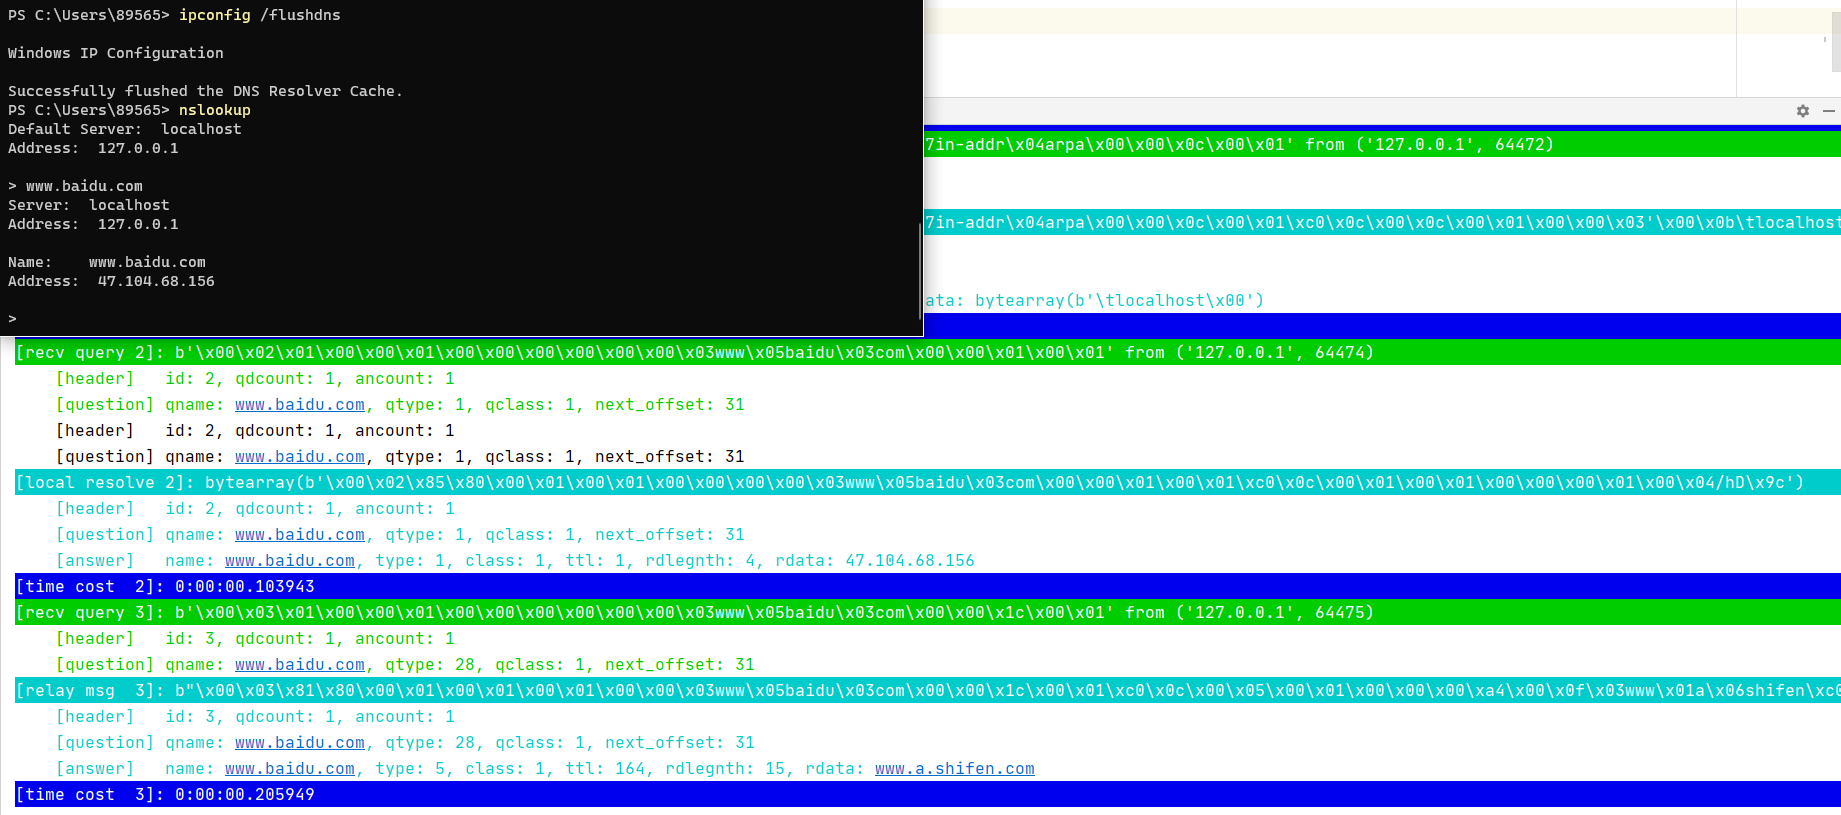
\includegraphics[width=\linewidth/9*8]{nsl_baidu.png}
	\caption{nslookup 查询 www.baidu.com 的结果}
\end{figure}\par
\item 查询 \hlg{picb.zhiming.com} 的结果: 按照要求, 利用让 rcode = 3 来返回查找不到, 如下图:
\begin{figure}[H]
	\centering
	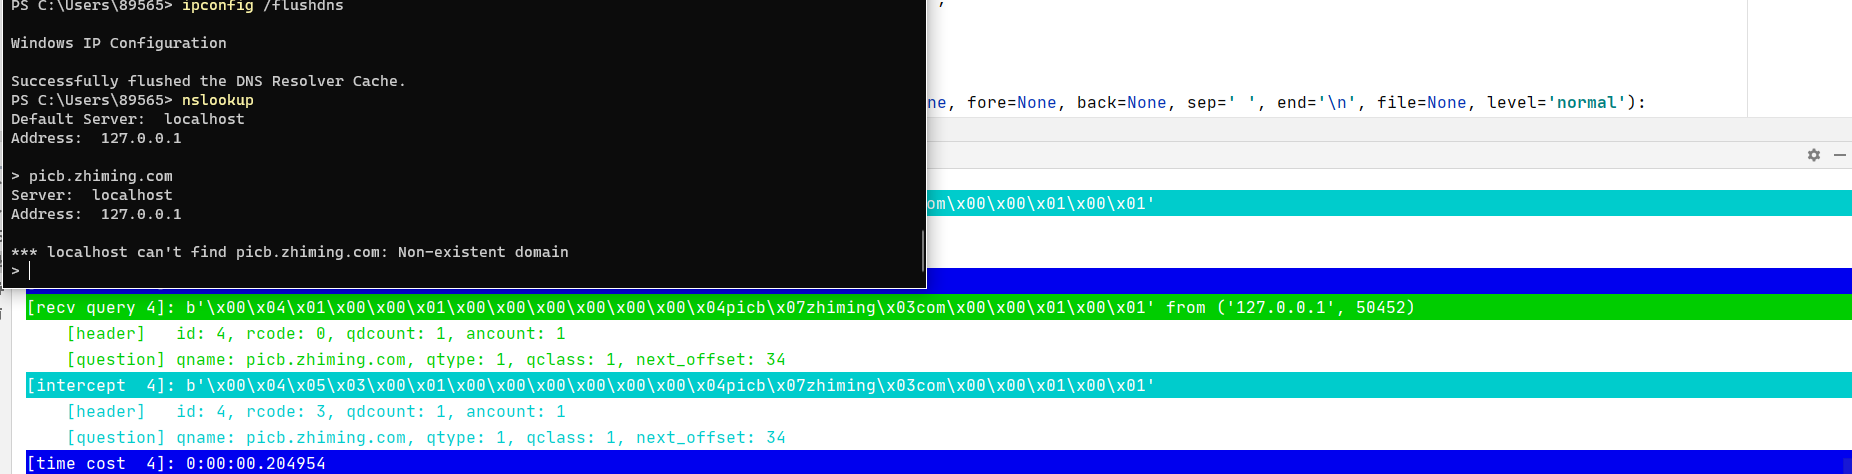
\includegraphics[width=\linewidth/9*8]{nsl_zhiming.png}
	\caption{nslookup 查询 picb.zhiming.com 的结果}
\end{figure}\par
\item 查询 \hlg{www.4399.com} 的结果: 此时它不在 config 文件中, 因此就进行 relay.
\begin{figure}[H]
	\centering
	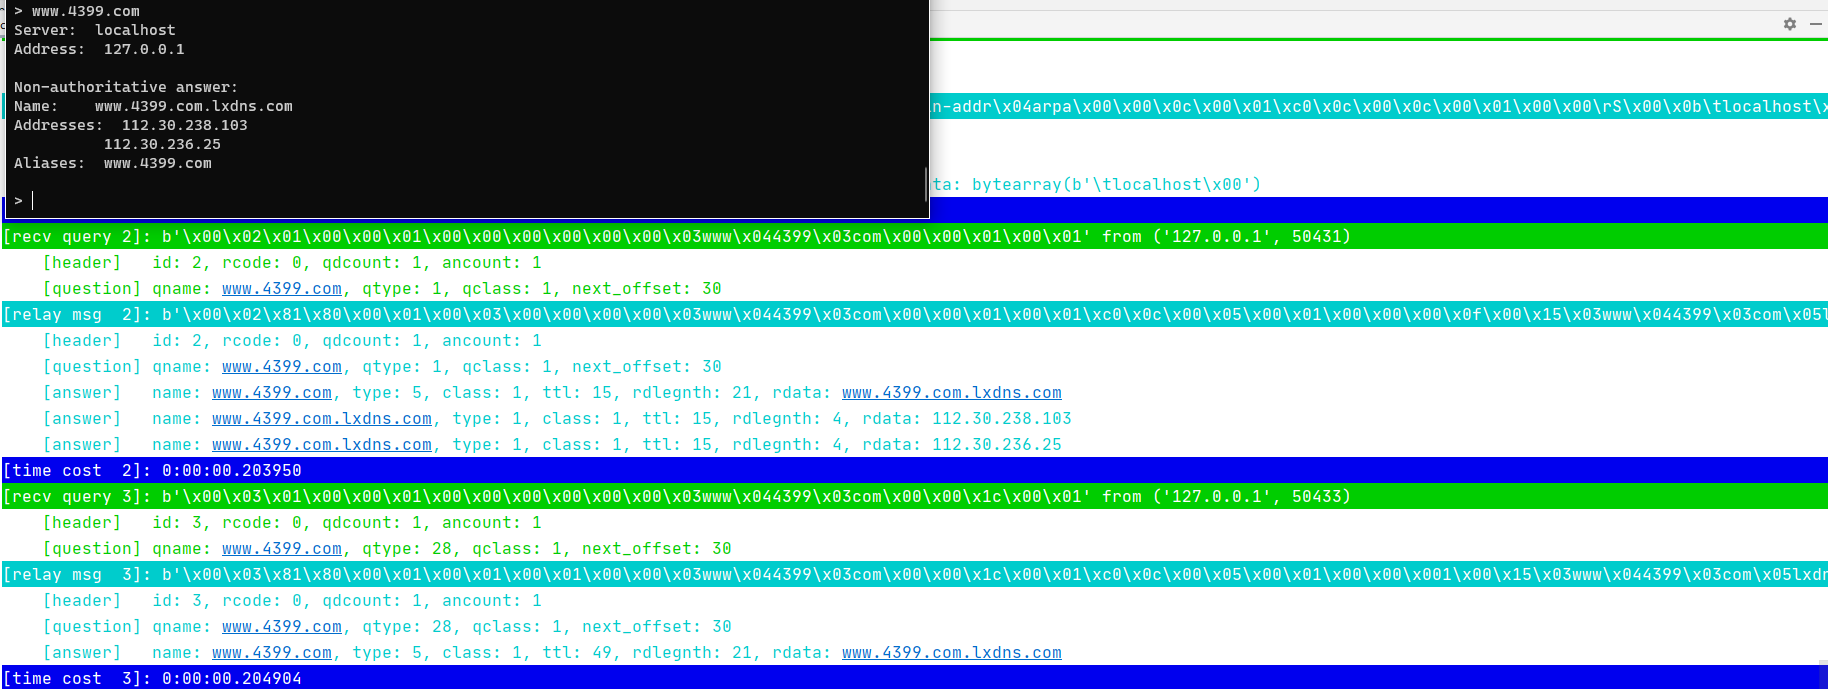
\includegraphics[width=\linewidth/9*8]{nsl_4399.png}
	\caption{nslookup 查询 www.4399.com 的结果}
\end{figure}\par
\end{itemize}
\subsection{Web Browser}
\subsubsection{知乎网页广告测试}
\noindent 为了测试知乎的广告, 使用以下配置:
\begin{figure}[H]
	\centering
	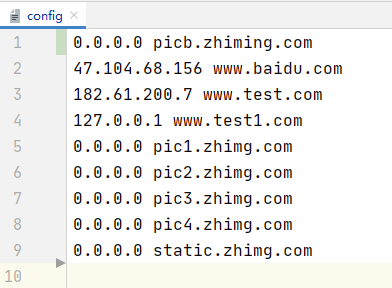
\includegraphics[width=\linewidth/2]{browser_config.png}
	\caption{Web Browser 测试的 config 文件}
\end{figure}\par
然后打开知乎, 会发现广告的图片的网址被 intercept:\\
\begin{figure}[H]
	\centering
	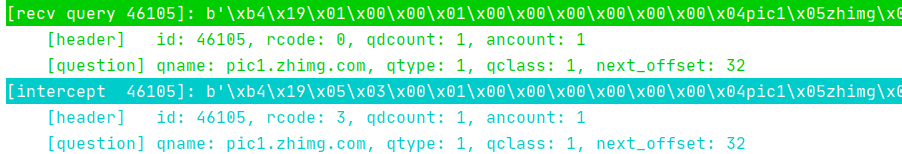
\includegraphics[width=\linewidth/9*8]{zhihu_output.png}
	\caption{访问知乎首页的输出效果}
\end{figure}\par
从而使浏览器无法收到广告的图片无法接受, 最终使得广告无法显示:\\
\begin{minipage}{\linewidth/2}
\begin{figure}[H]
	\centering
	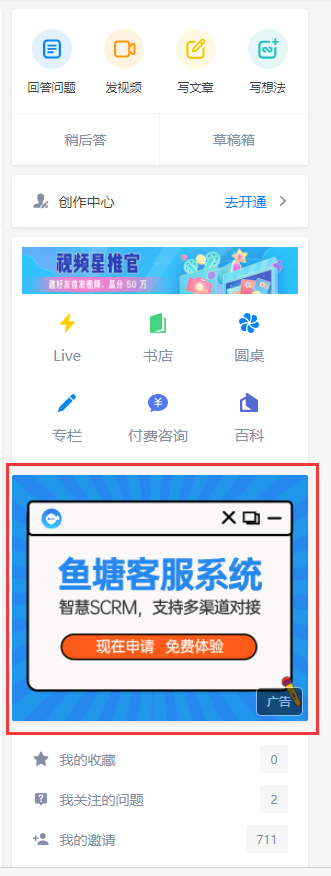
\includegraphics[width=\linewidth/3*2]{zhihu_ad.png}
	\caption{去除广告前的知乎(红线框出)}
\end{figure}\par
\end{minipage}
\begin{minipage}{\linewidth/2}
\begin{figure}[H]
	\centering
	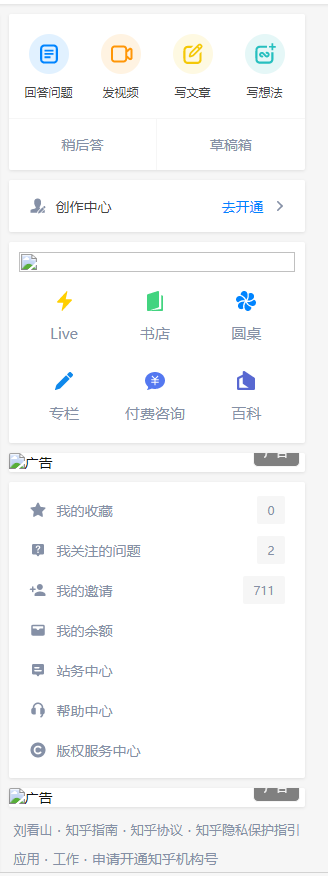
\includegraphics[width=\linewidth/3*2]{zhihu_noad.png}
	\caption{去除广告后的知乎}
\end{figure}\par
\end{minipage}
\subsubsection{7K7K 网页图片测试}
同理, 
\begin{figure}[H]
	\centering
	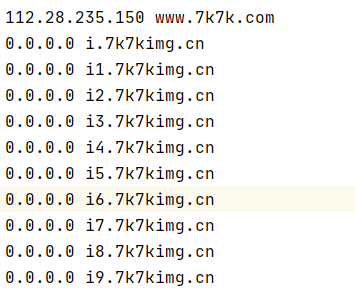
\includegraphics[width=\linewidth/3]{7k7k_config.png}
	\caption{Web Browser 测试的 7k7k config 文件}
\end{figure}\par
\begin{figure}[H]
	\centering
	
\includegraphics[width=\linewidth/3*2]{7k7k.png}
	\caption{去除图片前的 7k7k}
\end{figure}\par
\begin{figure}[H]
	\centering
	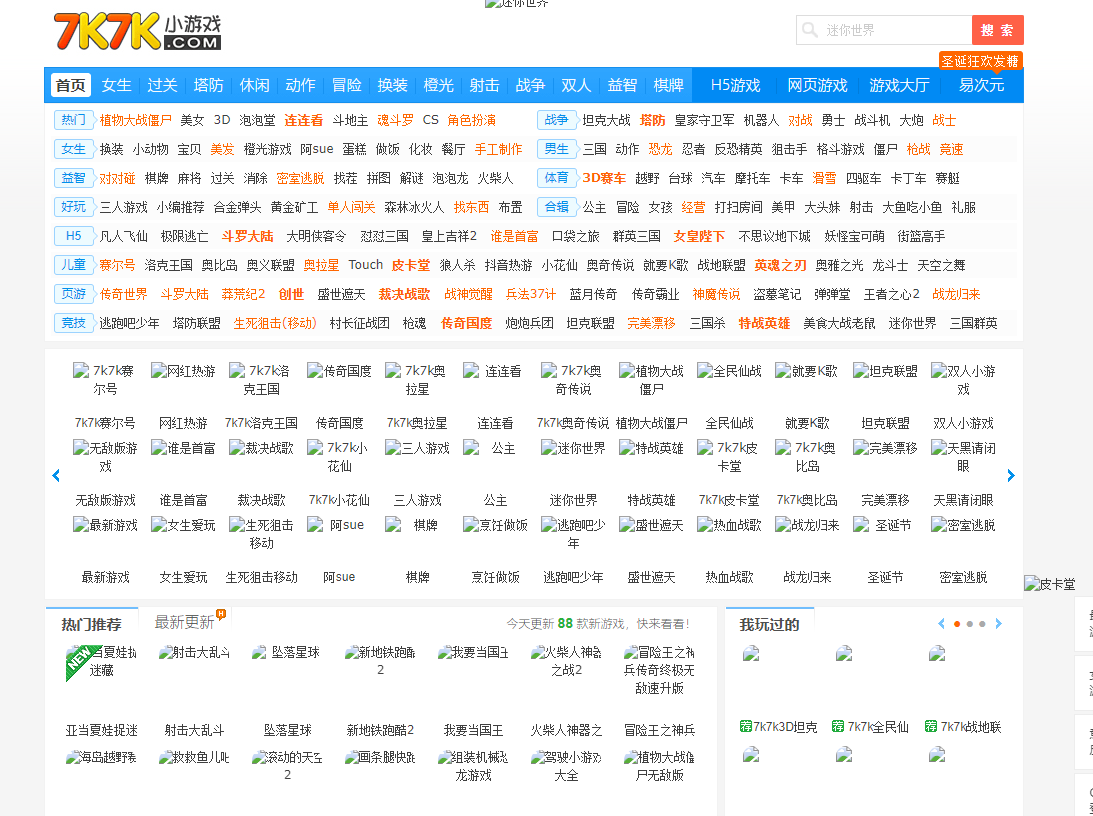
\includegraphics[width=\linewidth/3*2]{7k7k_ad.png}
	\caption{去除图片后的 7k7k}
\end{figure}\par
\subsubsection{CSDN 网页广告测试}
同理, 
\begin{figure}[H]
	\centering
	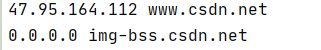
\includegraphics[width=\linewidth/3]{csdn_config.png}
	\caption{Web Browser 测试的 csdn config 文件}
\end{figure}\par
\begin{figure}[H]
	\centering
	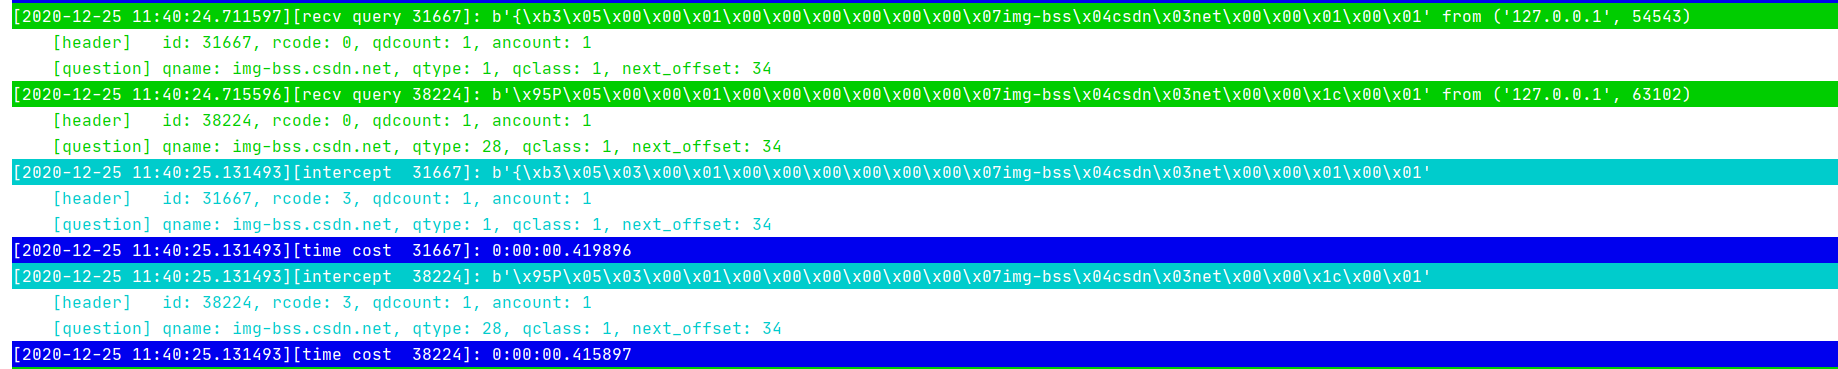
\includegraphics[width=\linewidth/9*8]{csdn_console.png}
	\caption{访问知乎首页的输出效果}
\end{figure}\par
\begin{figure}[H]
	\centering
	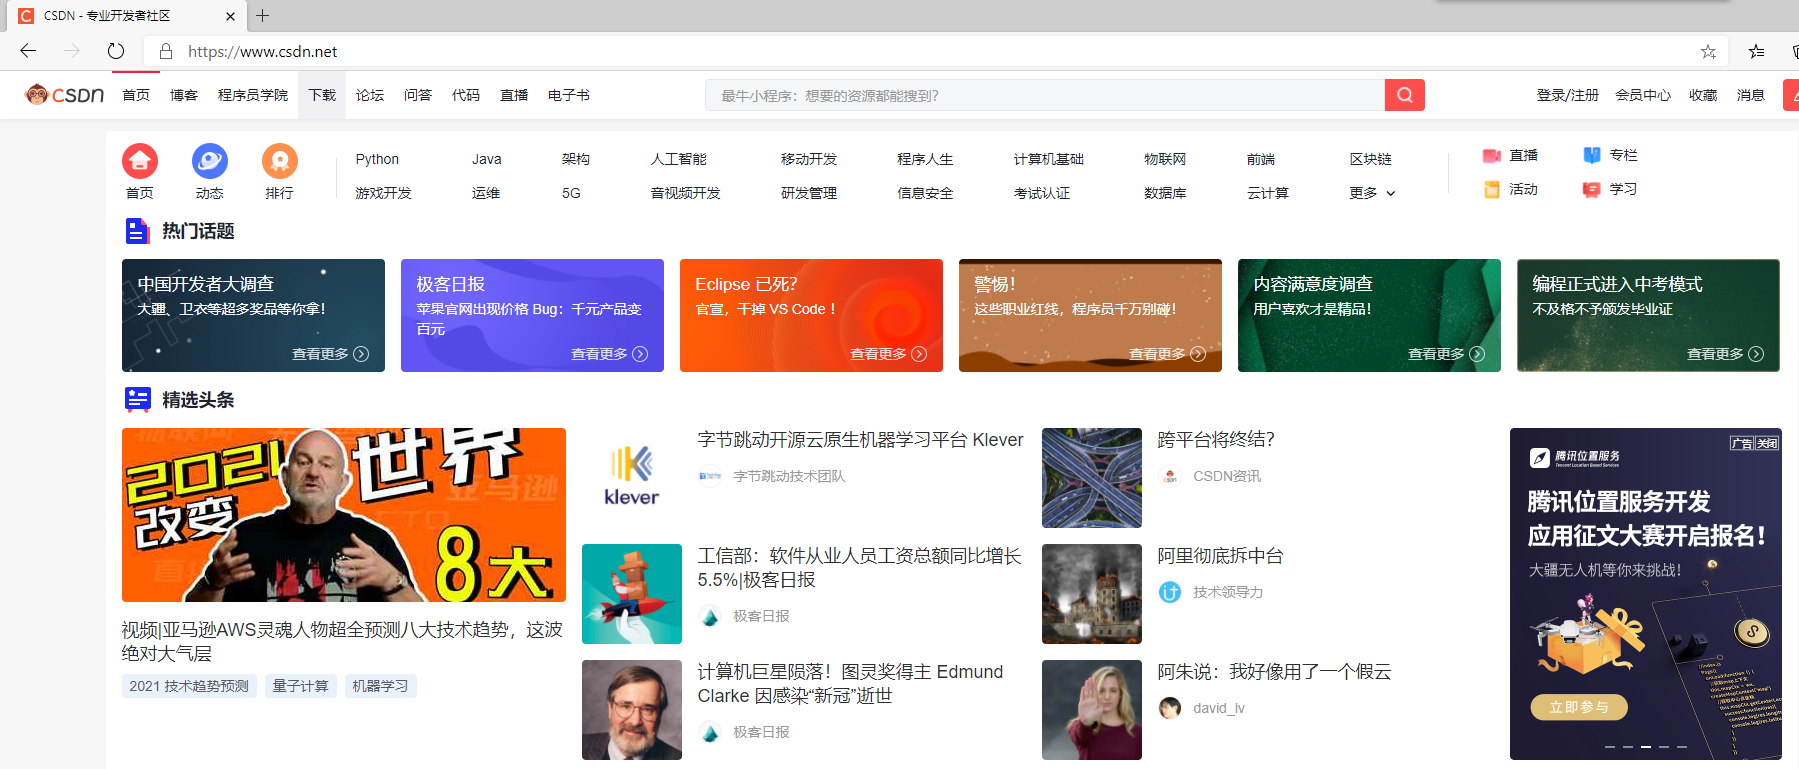
\includegraphics[width=\linewidth/3*2]{csdn.png}
	\caption{去除广告前的 csdn}
\end{figure}\par
\begin{figure}[H]
	\centering
	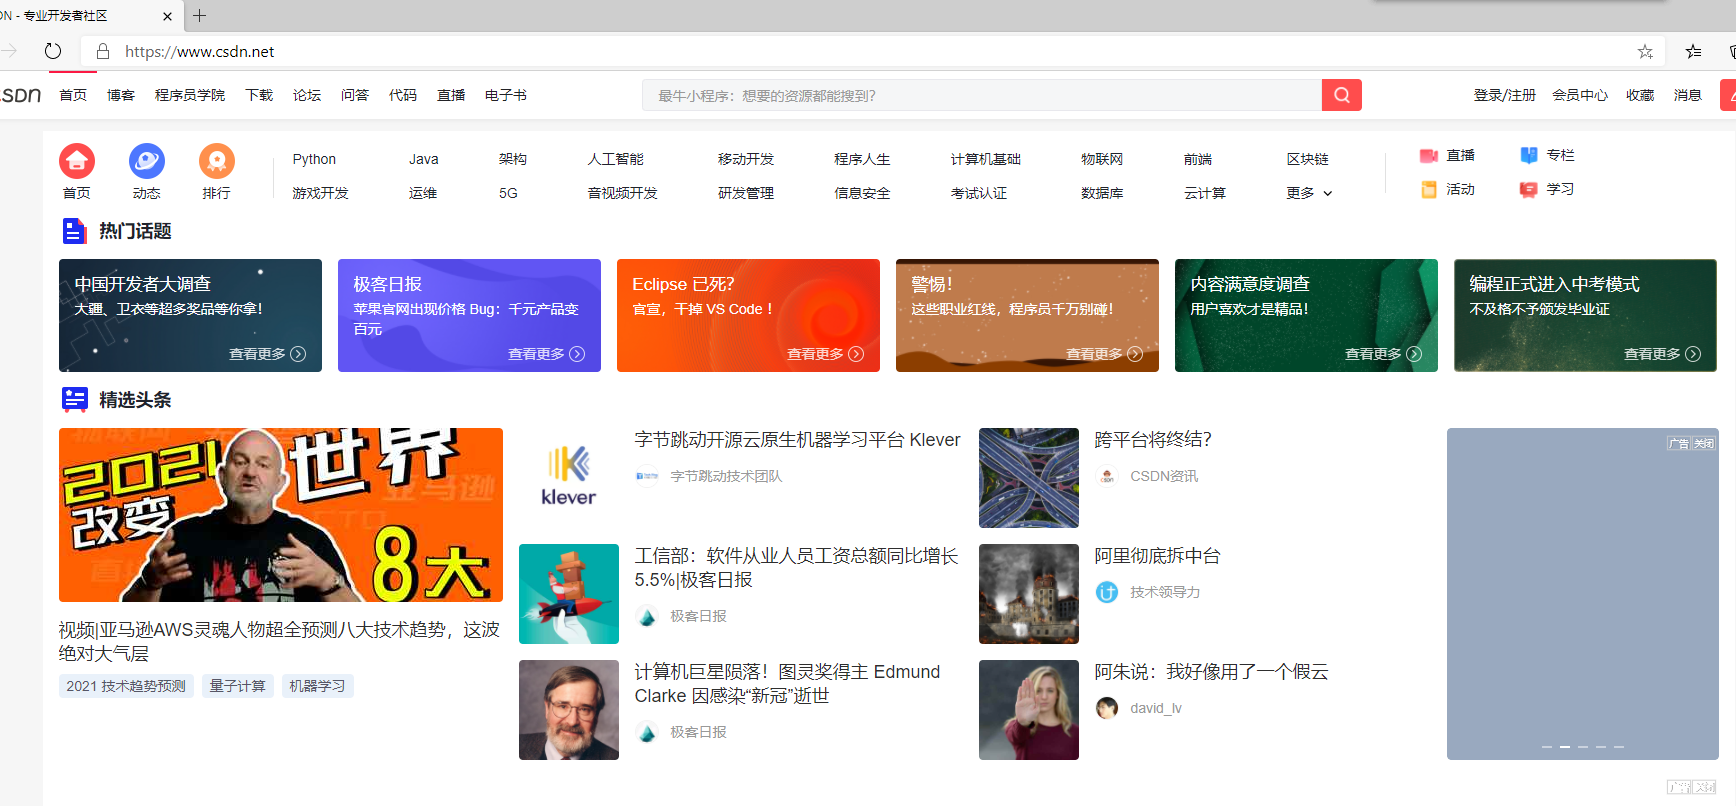
\includegraphics[width=\linewidth/3*2]{csdn_ad.png}
	\caption{去除广告(屏幕右侧)后的 csdn}
\end{figure}\par

\section{实验总结}
\noindent 本次实验中, 不仅更深刻地了解了 DNS 请求的相关协议, 且也更熟悉了 Python 的代码编写, 包括但不限于其 socket, multiprocessing 的使用等, 收获颇丰.






\end{document}














